\documentclass[12pt,a4paper,oneside]{book} 
\usepackage[utf8]{inputenc}
\usepackage[spanish]{babel}
\usepackage{amsmath}
\usepackage{amsfonts}
\usepackage{amssymb}
\usepackage[backend=biber]{biblatex}
\bibliography{referencias}
\usepackage{abstract} % Allows abstract customization
\renewcommand{\abstractnamefont}{\normalfont\bfseries} % Set the "Abstract" text to bold
\renewcommand{\abstracttextfont}{\normalfont\small\itshape} % Set the abstract itself to small italic text


\usepackage{amssymb, amsmath}
\usepackage{graphicx}
\usepackage[left=2.54cm,right=2.54cm,top=2.54cm,bottom=2.54cm]{geometry}

\begin{document}
	
	\thispagestyle{empty} 
	
	\begin{center} 
		\LARGE{UNIVERSIDAD PRIVADA DE TACNA} \\[0.5cm] 
		\Large{FACULTAD DE INGENIER\'IA DE SISTEMAS}\\[0.5cm] 
		\large{ ESCUELA PROFESIONAL DE INGENIER\'IA SISTEMAS} 
	\end{center}
	
	\begin{figure}[htb]
		\centering 
\includegraphics[width=6cm, height=7cm]{img/uptlogo.jpg}
	\end{figure}
	
	\begin{center} 
		\LARGE{\bf Trabajo encargado N-01 }\\
		\LARGE{\bf Comparativa de la estructura de datos de gestores de base de datos no relacionales }\\ \vspace{.25cm}
		
	\end{center}
	
	\begin{center} 
		
		\textbf {CURSO}\\ 
		\large Base de Datos II \\
		
		\textbf {DOCENTE}\\
		\large Mag. Patrick Cuadros Quiroga\\
		
		\textbf {INTEGRANTES}\\
		\large Limache Victorio, V\'ictor Piero  \\
		\large Sanchez Rodriguez, Bayron  \\
		\large Tarqui Montalico, Risther  \\
		\large Callata Flores, Rafael \\
		\large Liendo Velasquez, Joaquin \\
		
	\end{center}
	
	\begin{center} 
		\Large \textsc{Tacna - Perú} \\
		\Large \textsc{2020 } 
	\end{center}
	
	
	
	\newpage
	
	
	
	%%INICIO abstract
	\begin{abstract}
		
	
		
		En este articulo analizaremos 2 tipos de base de datos, el relacional(SQL) y el No relacional (NoSQL). Conoceremos las definiciones, características, aplicaciones, comparativas de 2  base de datos como ejemplo en el SQL y  también en el NoSQL, entre otras características. También, se hace una comparativa entre los tipos de base de datos tomando como criterio: cargas de trabajo óptimas, modelo de datos, propiedades ACID, rendimiento y el escalado API. Finalmente se llega a conclusiones tomando en cuenta todo lo anteriormente analizado.\\ 	
		
		Reflexiona sobre las bases de datos NoSQL, describiéndolas y analizando el porqué de su importancia y actualidad; además recopila y define algunas características de este tipo de base de datos, para revisar las taxonomías más importantes y analizar el uso conjunto de tecnologías NoSQL y relacionales, con el fin de proporcionar un punto de partida para los trabajos en esta área por parte de investigadores.\\ 
		
		\begin{center}
			
			\textbf{Abstract}
		\end{center}
	
		In this article we will analyze 2 types of database, the relational (SQL) and the Non-relational (NoSQL). We will know the definitions, characteristics, applications, comparisons of 2 databases as an example in SQL and also in NoSQL, among other characteristics. Also, a comparison is made between the types of databases taking as criteria: optimal workloads, data model, ACID properties, performance and API scaling. Finally, conclusions are reached taking into account everything previously analyzed.\\ 
	
		He reflects on NoSQL databases, describing them and analyzing why they are important and current; It also collects and defines some characteristics of this type of database, to review the most important taxonomies and analyze the joint use of NoSQL and relational technologies, in order to provide a starting point for researchers' work in this area.\\ 
		
		
	\end{abstract}
	%%FIN abstract
	
	
	\newpage
	
	\begin{center}
		\texttt{Comparativa de la estructura de datos de gestores de base de datos no relacionales} 
	\end{center}
	
	\begin{enumerate}
		\item Introducción
		
		Son muchas las aplicaciones web que utilizan algún tipo de bases de datos para funcionar. Hasta ahora estábamos acostumbrados a utilizar bases de datos SQL como son MySQL, Oracle o MS SQL, pero desde hace ya algún tiempo han aparecido otras que reciben el nombre de NoSQL (Not only SQL – No sólo SQL) y que han llegado con la intención de hacer frente a las bases relacionales utilizadas por la mayoría de los usuarios.\\
		
		Es muy común que los desarrolladores de software estemos en la situación de elegir entre bases de datos relacionales y no relacionales. No es para verlo como un dilema o pensar que dependiendo de la decisión vamos a fracasar, en realidad con cualquiera de las dos opciones, es posible construir nuestro sistema, dependiendo de lo que queramos.\\
		
		Entonces surgen diferentes interrogantes: ¿Es importante saber las diferencias entre ambas bases de datos? ¿Cuál deberíamos usar en cada caso? Estas son preguntas bastante interesantes, puesto que un buen diseño de la base de datos es un factor de alta influencia con respecto a la calidad del proyecto. Dependiendo de la naturaleza de éste, se debe elegir la base de datos, ya que las dos tienen diferentes características.\\
		
		Para empezar con  un poco de historia, las bases de datos relacionales se comenzaron a utilizar en los años 80; a diferencia de las no relacionales que se están empezando a usar y tuvieron un importante crecimiento entre 2012 y 2015. Sin embargo, hoy sigue siendo más popular la primera opción.\\
		
		
		\item Desarrollo
		
		\texttt{Base de datos no relacionales} 
		
		\begin{enumerate}
			\item ¿Que son las bases de datos NoSQL?\\
			
			Se puede decir que la aparición del término NoSQL aparece con la llegada de la web 2.0 ya que hasta ese momento sólo subían contenido a la red aquellas empresas que tenían un portal, pero con la llegada de aplicaciones como Facebook, Twitter o YouTube, cualquier usuario podía subir contenido, provocando así un crecimiento exponencial de los datos.\\
			
			Es en este momento cuando empiezan a aparecer los primeros problemas de la gestión de toda esa información almacenada en bases de datos relacionales. En un principio, para solucionar estos problemas de accesibilidad, las empresas optaron por utilizar un mayor número de máquinas, pero pronto se dieron cuenta de que esto no solucionaba el problema, además de ser una solución muy cara. La otra solución era la creación de sistemas pensados para un uso específico que con el paso del tiempo han dado lugar a soluciones robustas, apareciendo así el movimiento NoSQL.\\
			
			Por lo tanto, hablar de bases de datos NoSQL es hablar de estructuras que nos permiten almacenar información en aquellas situaciones en las que las bases de datos relacionales generan ciertos problemas debido principalmente a problemas de escalabilidad y rendimiento de las bases de datos relacionales donde se dan cita miles de usuarios concurrentes y con millones de consultas diarias.\\
			
			Además de lo comentado anteriormente, las bases de datos NoSQL son sistemas de almacenamiento de información que no cumplen con el esquema entidad–relación. Tampoco utilizan una estructura de datos en forma de tabla donde se van almacenando los datos, sino que para el almacenamiento hacen uso de otros formatos como clave–valor, mapeo de columnas o grafos (ver epígrafe ‘Tipos de bases de datos NoSQL’).\\
			
			
			\item Ventajas de los sistemas NoSQL.\\
			Esta forma de almacenar la información ofrece ciertas ventajas sobre los modelos relacionales. Entre las ventajas más significativas podemos destacar:\\
			\begin{enumerate}
				\item Se ejecutan en máquinas con pocos recursos: Estos sistemas, a diferencia de los sistemas basados en SQL, no requieren de apenas computación, por lo que se pueden montar en máquinas de un coste más reducido. 	\\
				\item Escalabilidad horizontal: Para mejorar el rendimiento de estos sistemas simplemente se consigue añadiendo más nodos, con la única operación de indicar al sistema cuáles son los nodos que están disponibles.
				\item Pueden manejar gran cantidad de datos: Esto es debido a que utiliza una estructura distribuida, en muchos casos mediante tablas Hash.\\
				\item No genera cuellos de botella: El principal problema de los sistemas SQL es que necesitan transcribir cada sentencia para poder ser ejecutada, y cada sentencia compleja requiere además de un nivel de ejecución aún más complejo, lo que constituye un punto de entrada en común, que ante muchas peticiones puede ralentizar el sistema.\\
			\end{enumerate}
		
				\begin{figure}[htb]
					\centering 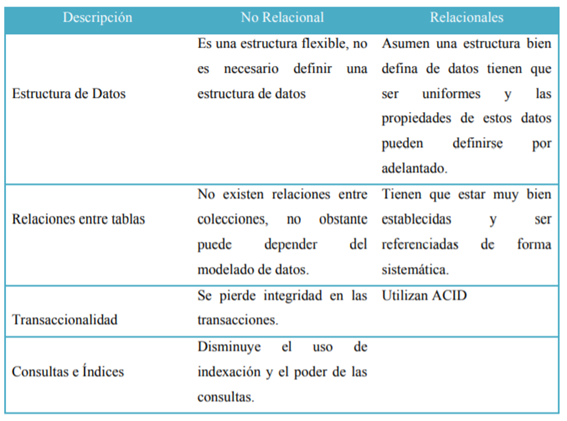
\includegraphics[width=12cm, height=9cm]{img/ventajas.png}
				\end{figure}
			\item Características\\
			Aunque es difícil determinar propiedades comunes para un conjunto de tecnologías, se proponen seis características específicas para poder encasillar a las
			bases de datos NoSQL:\\
			
			\begin{enumerate}
				\item Escalabilidad horizontal: refiriéndose a la facilidad añadir, eliminar o realizar operaciones con elementos (hardware) del sistema, sin afectar el rendimiento.
				\item Habilidad de distribución: tiene que ver con la escalabilidad horizontal, pero haciendo énfasis en su soporte; para ello se tiene en cuenta la habilidad de replicar y distribuir los datos sobre los servidores.
				\item Uso eficiente de recursos: aprovecha las nuevas tecnologías, como los discos en estado sólido, el uso eficiente de recursos como la memoria RAM y los sistemas distribuidos en general.
				\item Libertad de esquema: al no tener un esquema rígido se permite mayor libertad para modelar los datos; además facilita la integración con los lenguajes de programación orientados a objetos, lo que evita el proceso de mapeado.
				\item Modelo concurrencia débil: no implementa ACID (Atomicity, Consistency, Isolation and Durability), que reúne las características necesarias para que una serie de ser consideradas una transacción, sin embargo, sí se tienen en cuenta algunas consideraciones para asegurar estos aspectos, pero no son tan estrictas.
				\item Consultas simples: las consultas requieren menos operaciones y son más naturales, por la tanto, se gana en simplicidad y eficiencia
			\end{enumerate}
			\item Base de datos NoSQL
			\begin{itemize}
				\item MongoDB \\
				Estamos ante el sistema gestor de bases de datos no relacionales más popular y utilizado actualmente.\\
				MongoDB es un SGBD NoSQL orientado a ficheros que almacena la información en estructuras BSON con un esquema dinámico que permite su facilidad de integración.\\
				Empresas como Google, Facebook, eBay, Cisco o Adobe utilizan MongoDB como sistema gestor de bases de datos.\\
				Las principales características de MongoDB son:
				
				\begin{itemize}
					\item Indexación y replicación
					\item Balanceo de carga.
					\item Almacenamiento en ficheros
					\item Consultas ad hoc
					\item Escalabilidad horizontal
					\item Open Source
				\end{itemize}
				Como desventaja principal, Mongo DB no es un SGBD adecuado para realizar transacciones complejas.\\
				\item Apache Cassandra\\
				Al igual que Redis (Otro SGBD conocido) Cassandra tambien utiliza almacenamiento clave-valor. Es un SGBD NoSQL distribuido y masivamente escalable.
				Empresas como Facebook, Twitter, Instagram, Spotify o Netflix utilizan Cassandra.\\
				Dispone de un lenguaje propio para las consultas denominado CQL (Cassandra Query Languaje).\\
				Las principales características de Cassandra son:\\
				\begin{itemize}
					\item Multiplataforma
					\item Propio lenguaje de consultas (CQL)
					\item Escalado lineal y horizontal
					\item Es un SGBD distribuido
					\item Utiliza una arquitectura peer-to-peer.
				\end{itemize}
				
				
		
			\end{itemize}
			\item Comparación
	
				\begin{figure}[htb]
					\centering 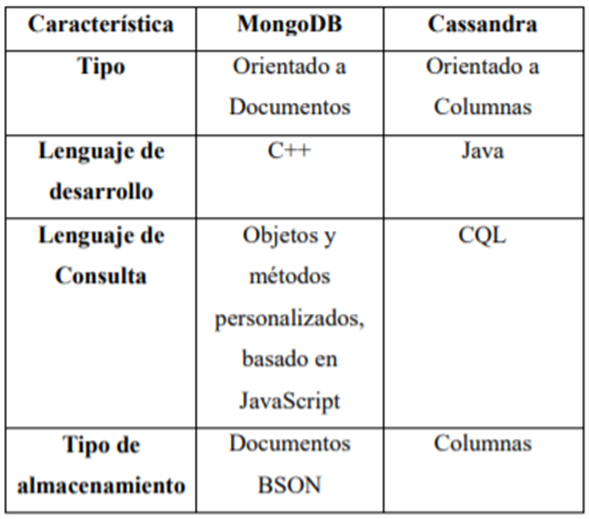
\includegraphics[width=12cm, height=12cm]{img/comparacion1.png}
				\end{figure}
			\newpage
				\begin{figure}[htb]
					\centering 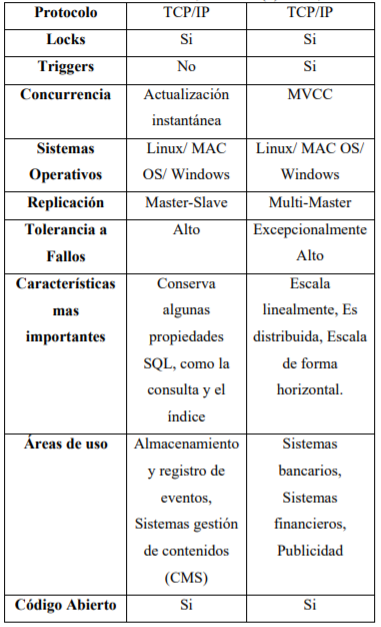
\includegraphics[width=12cm, height=18cm]{img/comparacion2.png}
				\end{figure}
		
		
		
		
		Mediante el análisis de las propiedades básicas, es posible concluir que existen similitudes cuando se trata de tipos de archivos utilizados, consultas, transacciones, locks, almacenamiento de datos, código abireto y sistemas operativos. \\
		
		En cuanto a términos de uso, MongoDB tiene un mejor uso para Sistemas de Gestion de Contenidos (CMS), mientras tiene consultas dinámicas con datos escritos frecuentemente. Cassandra está optimizado para almacenar e interactuar con grandes cantidades de datos que se pueden utilizar en diferentes áreas, tales como, finanzas o publicidad.\\
		
		\texttt{Base de datos relacionales} \\
		
		\begin{enumerate}
			\item Definición
		
				Una base de datos relacional es una recopilación de elementos de datos con relaciones predefinidas entre ellos. Estos elementos se organizan como un conjunto de tablas con columnas y filas. \\
				
				Las tablas se utilizan para guardar información sobre los objetos que se van a representar en la base de datos. Cada columna de una tabla guarda un determinado tipo de datos y un campo almacena el valor real de un atributo.\\ 
				
				Las filas de la tabla representan una recopilación de valores relacionados de un objeto o una entidad. \\
				
				Cada fila de una tabla podría marcarse con un identificador único denominado clave principal, mientras que filas de varias tablas pueden relacionarse con claves extranjeras. Se puede obtener acceso a estos datos de muchas formas distintas sin reorganizar las propias tablas de la base de datos.\\
				
			\item Origenes
		
				Uno de los primeros modelos de bases de datos fue el modelo jerárquico, en el que los datos se organizan con una estructura de árbol similar a la de los sistemas de archivos modernos. \\
				
				El siguiente ejemplo muestra el aspecto que podría tener el diseño de una parte de una base de datos jerárquica utilizada para categorizar animales:\\
				
				\begin{figure}[htb]
					\centering 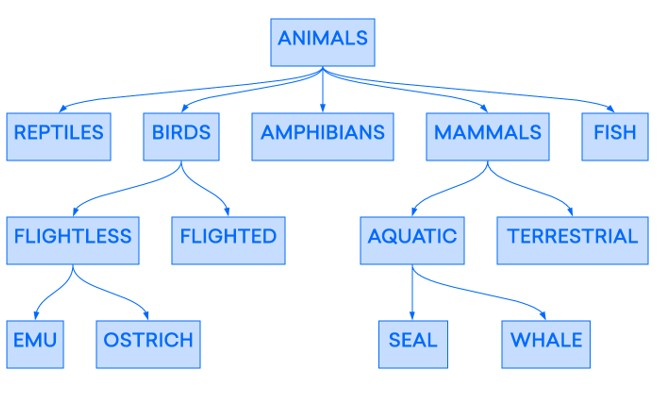
\includegraphics[width=12cm, height=7cm]{img/NoSQL/1.jpg}
				\end{figure}
			
			A fines de los años 60, Edgar F. Codd, un especialista en ciencias de la computación que trabajaba en IBM, diseñó el modelo relacional de administración de bases de datos. El modelo relacional de Codd permitía que los registros individuales se relacionaran con más de una tabla y, de esta manera, posibilitaba las relaciones “varios a varios” entre los puntos de datos además de las relaciones “uno a varios”. Esto proporcionó más flexibilidad que los demás modelos existentes a la hora de diseñar estructuras de base de datos y permitió que los sistemas de gestión de bases de datos relacionales (RDBMS) pudieran satisfacer una gama mucho más amplia de necesidades empresariales.\\
				
			\item ¿Cómo se estructuran las bases de datos relacionales?
			
			La distinción entre lógica y física también se aplica a las operaciones de la base de datos, que son acciones claramente definidas que permiten a las aplicaciones manipular los datos y las estructuras de la base de datos. Las operaciones lógicas permiten que una aplicación especifique el contenido que necesita, mientras que las operaciones físicas determinan cómo se debe acceder a esos datos y luego realizan la tarea.\\
			
			Para garantizar que los datos sean siempre precisos y accesibles, las bases de datos relacionales siguen ciertas reglas de integridad. Por ejemplo, una regla de integridad puede especificar que no se permitan filas duplicadas en una tabla, para eliminar la posibilidad de que ingrese información errónea en la base de datos.\\
			
			\begin{figure}[htb]
				\centering 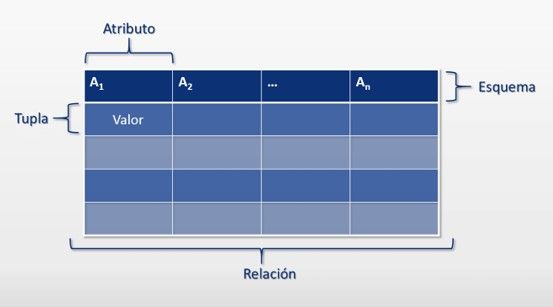
\includegraphics[width=12cm, height=7cm]{img/NoSQL/2.jpg}
			\end{figure}
			
			\item Ventajas y Desventajas de las Bases de Datos SQL
					\begin{itemize}
						\item Ventajas
						
						\begin{enumerate}
						
							\item Portabilidad: SQL puede ser usado en laptops, computadoras, servidores o dispositivos móviles.
							\item Experiencia y madurez: Este es uno de sus puntos más fuertes. El tiempo y la aceptación generalizada de los desarrolladores ha permitido crear gran cantidad de información y herramientas en torno a ellas.
							\item Atomicidad: Los desarrolladores generalmente se ven dispuestos a inclinarse por los modelos relacionales gracias a la atomicidad. Esto significa que cualquier operación que se quiera ejecutar y no cumpla con los criterios de información preestablecidos, no se realizará.
							\item Estándares bien definidos: Todos los procesos deben estar bajo los estándares que plantea el SQL. Brindando de esta forma criterios de uniformidad a la información.
							\item Escritura simple: Gran parte de la aceptación depende de la sencillez de su método de escritura. Este es muy parecido al lenguaje que utilizamos los humanos, facilitando para nosotros la comprensión de las operaciones.
							
						\end{enumerate}
						
						\item Desventajas
						
						\begin{enumerate}
							
							\item Dificultades de crecimiento: Cuando estas bases de datos comienzan a crecer en volumen, el almacenamiento y el costo de mantenimiento se convierten en un problema de alto costo.
							\item Cambios en la estructura: el entorno empresarial es altamente dinámico. Esto exige que se realicen cambios de forma eventual en los registros de datos. Si ejecutamos cambios, la Base de Datos debe ser modificada en su estructura para admitir las modificaciones. Si las modificaciones no se realizan esta se verá afectada y sus procesos interrumpidos.
							\item Complejidad en la instalación: Algunas bases de datos SQL se ven condicionadas por el sistema operativo en el cual van a funcionar y los requisitos mínimos de funcionamiento de los servidores u ordenadores.
							\item Dificultad en la interfaz: La interfaz de una base de datos SQL son más complejas que agregar algunas líneas de código.
							\item Más características implementadas de forma patentada: Aunque las bases de datos SQL se ajustan a los estándares ANSI e ISO, algunas bases de datos implementan extensiones propietarias al SQL estándar para garantizar el bloqueo del proveedor.
							
						\end{enumerate}
					
					\end{itemize}
			\item Caracteristicas
				\begin{enumerate}
					
					\item Una base de datos relacional se compone de varias tablas o relaciones. 
					\item No pueden existir dos tablas con el mismo nombre ni registro. 
					\item Cada tabla es a su vez un conjunto de registros (filas y columnas). 
					\item La relación entre una tabla padre y un hijo se lleva a cabo por medio de las claves primarias y ajenas (o foráneas). 
					\item Las claves primarias son la clave principal de un registro dentro de una tabla y éstas deben cumplir con la integridad de datos. 
					\item Las claves ajenas se colocan en la tabla hija, contienen el mismo valor que la clave primaria del registro padre
					
				\end{enumerate}
			\item ¿Qué buscar a la hora de seleccionar una base de datos relacional?\\
			
			Varios factores pueden guiar su decisión al momento de elegir entre tipos de bases de datos y productos de bases de datos relacionales. El RDBMS que elija dependerá de las necesidades de su negocio. Hágase las siguientes preguntas:\\
			
				\begin{enumerate}
					\item ¿Cuáles son nuestros requisitos de precisión de datos? ¿El almacenamiento de datos y la precisión dependerán de la lógica empresarial? ¿Nuestros datos tienen requisitos estrictos de precisión (por ejemplo, datos financieros e informes gubernamentales)?
					\item ¿Necesitamos escalabilidad? ¿Cuál es la escala de los datos a administrar y cuál es su crecimiento previsto? ¿Será necesario que el modelo de base de datos admita copias de base de datos duplicadas (como instancias separadas) para la escalabilidad? Si es así, ¿puede mantener la consistencia de los datos en esas instancias?
					\item ¿Qué tan importante es la concurrencia? ¿Varios usuarios y aplicaciones necesitarán un acceso simultáneo a los datos? ¿El software de la base de datos admite concurrencia mientras protege los datos?
					\item ¿Cuáles son nuestras necesidades de rendimiento y confiabilidad? ¿Necesitamos un producto de alto rendimiento y alta confiabilidad? ¿Cuáles son los requisitos para el rendimiento de la consulta-respuesta? ¿Cuáles son los compromisos de los proveedores para los acuerdos de nivel de servicio (SLA) o tiempo de inactividad no planificado?
					
				\end{enumerate}
		\end{enumerate}
		
		\item Comparativa de SQL y NoSQL
		
		\begin{figure}[htb]
			\centering 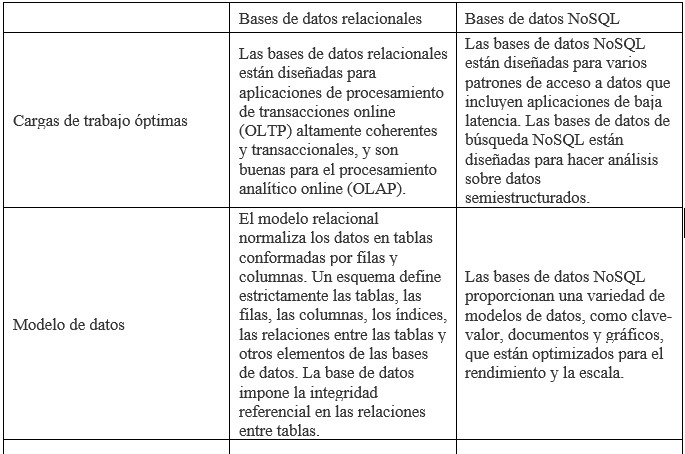
\includegraphics[width=12cm, height=7cm]{img/NoSQL/4.1.jpg}
		\end{figure}
	
		\begin{figure}[htb]
			\centering 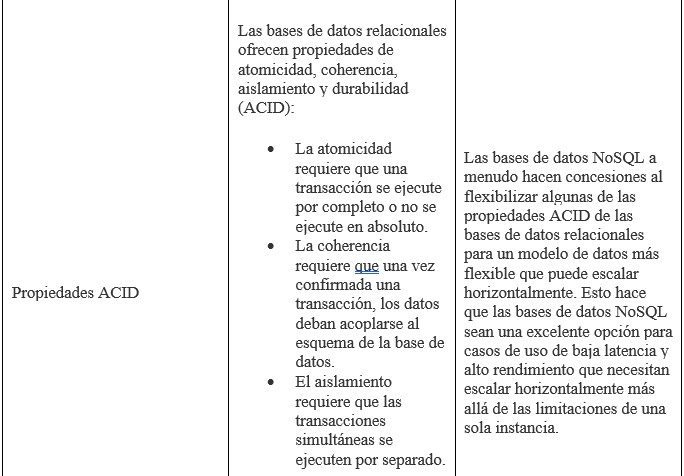
\includegraphics[width=12cm, height=7cm]{img/NoSQL/4.2.jpg}
		\end{figure}
	\newpage
		\begin{figure}[htb]
			\centering 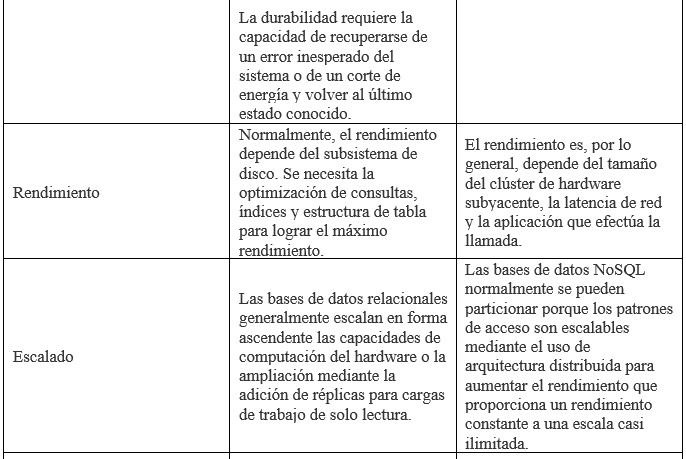
\includegraphics[width=12cm, height=7cm]{img/NoSQL/4.3.jpg}
		\end{figure}
		
		\begin{figure}[htb]
			\centering 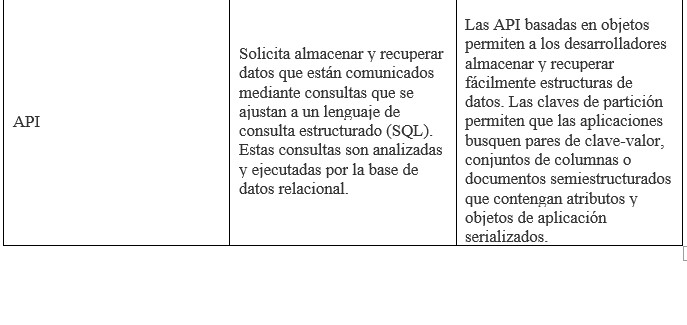
\includegraphics[width=12cm, height=5cm]{img/NoSQL/4.4.jpg}
		\end{figure}
			
		
		\end{enumerate}
		\item Conclusiones\\
		
		\begin{enumerate}
			\item Las base de datos NoSQL suelen ser mucho más abiertas y flexibles. Permiten adaptarse a necesidades de proyectos mucho más fácilmente que los modelos de Entidad Relación de SQL\\
			
			\item Las base de datos NoSQL surgieron  después de las SQL, por necesidades especificas de algunas empresas.\\
			
			\item Las bases de datos NoSQL generalmente procesan los datos más rápido que las bases de datos relacionales, se pueden hacer cambios de los esquemas sin tener que parar bases de datos y lo mejor de todo optimizan las consultas en base de datos para grandes cantidades de datos.\\
			
			\item SQL y NoSQL han sido grandes inventos a lo largo del tiempo para mantener el almacenamiento y la recuperación de datos optimizados y sin problemas. Criticar a cualquiera de ellos no ayudará a la causa. Si hay un zumbido de NoSQL en estos días, no significa que sea una bala de plata para todas sus necesidades. Ambas tecnologías son las mejores en lo que hacen. Corresponde al promotor hacer un mejor uso de ellos en función de las situaciones y necesidades.\\
			
			
		\end{enumerate}
		\item Recomendaciones
		
		Entre los SGBD citados encontraremos alguno que se adapte a nuestras necesidades de acuerdo a la inversión a realizar, el volumen de información a almacenar, el tipo de consulta a realizar, etc.\\
		
		\item Bibliografía
	
	
	https://www.acens.com/wp-content/images/2014/02/bbdd-nosql-wp-acens.pdf
	
	https\://es\.scribd\.com/document/384154812/Dialnet\-UtilidadYFuncionamientoDeLasBasesDeDatosNoSQL\-5029469\-pdf 
	
	https://prezi.com/h8jro-eyuscx/bases-de-datos-nosql/ 
	
	
	
	
	
		
	\end{enumerate}
	
	
	
\end{document}
